\chapter{Digital Geometry}
\label{chapter:digital-geometry}

The primitives of Euclidean geometry, such as lines and points, are idealized objects. A line segment is infinitely thin and a point is dimensionless. When referring to such entities, we eventually make use of visual representations and the line is incarnated as a trace and the point as a dot in the black board, for example. As long as we have the mathematical description of some shape $S$, we do not need any visual representation of it to compute its tangents, curvatures or perimeter. 

In imaging, however, it is almost always the case that we do not have a mathematical description of the objects in the scene. We need to identify the primitives from its visual representations.  We are not dealing with idealized objects anymore, but with finite descriptions of them. One of the subjects of study of digital geometry, and the one focused in this chapter, is how to correctly measure geometric properties in digitized objects.

We introduce basic concepts of digital geometry in~\cref{ch4:sec:ground-concepts} and we point out the difference between exact sampling and digitization. In~\cref{ch4:sec:geometric-measurements}, we introduce the multigrid convergence property and we give examples of several multigrid convergent estimators for local and global geometric measurements.

%As an illustration, consider the following examples of problems related with convex sets arising from each of this sub fields
%
%\begin{itemize}
%	\item[]{\textbf{Geometry}: What is the convex polygon of smallest area enclosing a shape $S$?}
%	\item[]{\textbf{Computational Geometry}: Given $n$ sample points of $S$, one can compute its convex hull in time $O(n \lg n)$.}
%	\item[]{\textbf{Discrete/Combinatorial geometry}: Take any $100$ convex sets in $R^2$ and denote them by $C_1, \cdots C_n$. If $C_i \cap C_j \cap C_k \neq \emptyset$, then $\bigcap C_i \neq \emptyset$.}
%	\item[]{\textbf{Digital geometry}: Let $D_h(S)$ be the digitization of a convex shape $S$. Can we devise a tangent estimator that is monotone with respect to some order in the digital boundary of $S$ for all its digitizations (different values of $h$)?}
%\end{itemize}


\section{Ground concepts}\label{ch4:sec:ground-concepts}

In this section, we define the grid point model and its adjacency relations. \revision{Together,} they allow us to define the digital line primitive. Next, we describe the grid intersection and Gauss digitization mappings, which link continuous objects to its digital representations in the grid point model. The concepts defined in this section can be explored in much more depth in the book~\cite{klette04digital}.

\subsection{Digital grid, digitization and digital line}

\begin{definition}{$2D$ Digital grid}
The $2D$ digital grid $h\mathbb{Z}^2 = \{ p = (h \cdot i,h \cdot j) \; | \; i,j \in \mathbb{Z}\}$ with grid step (resolution) $h \in \mathbb{R}_++ \setminus \{0\}$ is a regular sampling of the plane. Its members are called \emph{grid points}.
\end{definition}

We can think of the digital grid as a regular tessellation of the plane. The grid points are the center of the \emph{grid squares} (pixels). The other components, \emph{grid edges } and \emph{grid vertices} are illustrated in~\cref{ch4:fig:grid-point-model}. They form the \emph{grid point model} of the plane. Next, we define the two commonest adjacency relations in the grid point model.

\begin{figure}
\begin{minipage}{0.6\textwidth}
\center
\subfloat[Grid point model\label{ch4:fig:grid-point-model}]{
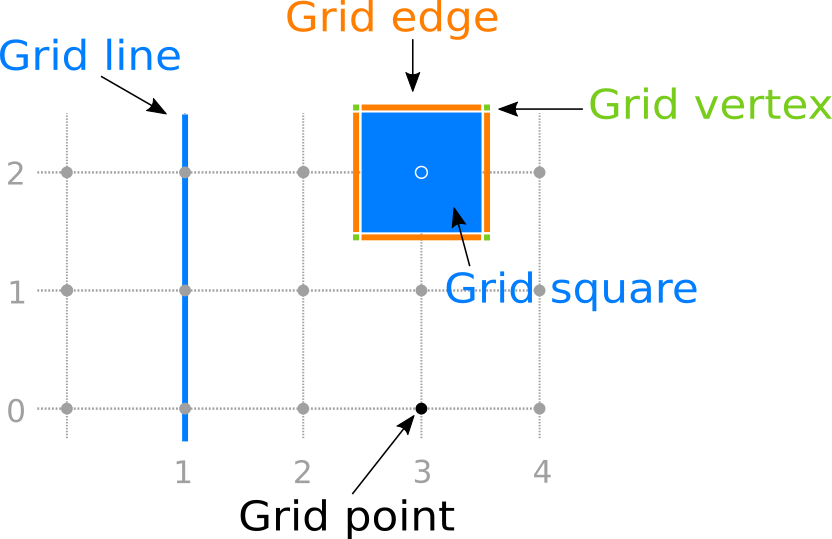
\includegraphics[scale=0.5]{figures/chapter4/digital-grid/grid-point-model.png}
}
\end{minipage}%
\begin{minipage}{0.4\textwidth}
\center
\subfloat[$4$-adjacency\label{ch4:fig:4-adjacency}]{
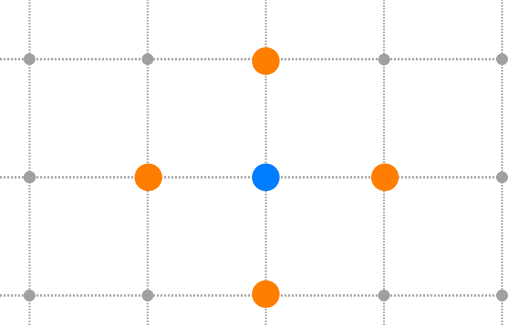
\includegraphics[scale=0.25]{figures/chapter4/digital-grid/4-adjacency.png}
}\hspace{1em}%
\subfloat[$8$-adjacency\label{ch4:fig:8-adjacency}]{
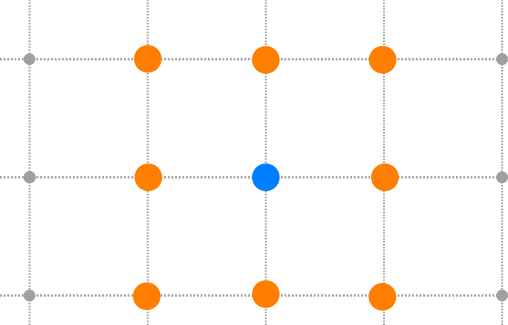
\includegraphics[scale=0.25]{figures/chapter4/digital-grid/8-adjacency.png}
}\\

\subfloat[Connected components\label{ch4:fig:connected-sets}]{
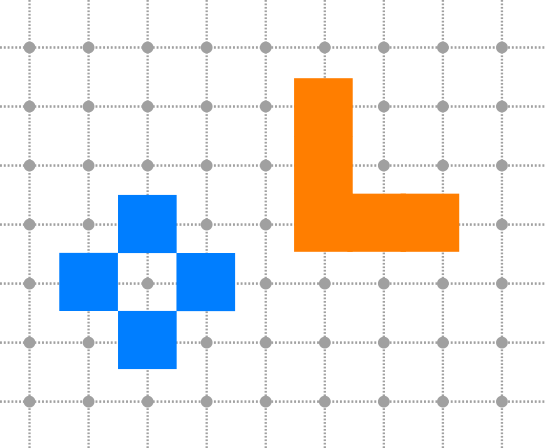
\includegraphics[scale=0.5]{figures/chapter4/digital-grid/connectivity.png}
}
\end{minipage}

\caption{\textbf{Digital grid and adjacency relations.} The grid point model and its components in (a); The $4$ and $8$ adjacency relations in (b) and (c); A $4$-connected set (orange) and a $8$-connected set (blue) in (d).}
\label{ch4:fig:digital-grid}
\end{figure}

\begin{definition}{$4$-adjacency relation}
Two grid points $p_1=(x_1,y_1)$ and $p_2=(x_2,y_2)$ are $4$-adjacent iff $p_1 \neq p_2$ and $|x_1-x_2| + |y_1-y_2| = 1$. We denote relation membership as $p_1A_4p_2$.
\end{definition}

\begin{definition}{$8$-adjacency relation}
Two grid points $p_1=(x_1,y_1)$ and $p_2=(x_2,y_2)$ are $8$-adjacent iff $p_1 \neq p_2$ and $\max \{ |x_1-x_2|, |y_1-y_2| \} = 1$. We denote relation membership as $p_1A_8p_2$.
\end{definition}

The adjacency relations are illustrated in~\cref{ch4:fig:4-adjacency,ch4:fig:8-adjacency}. Armed with an adjacency relation, we can define the notions of path and connectivity. A \emph{$4$-connected path} is a sequence $\{p_1,p_2,\cdots, p_n\}$ of grid points such that $p_iA_4p_{i+1}$ for all $1 \leq i < n$. A set $P$ is \emph{$4$-connected} if for every $p,q \in P$ there exists a $4$-connected path starting at $p$ and ending at $q$. Analogous definitions holds for $8$-adjacency relation~(see~\cref{ch4:fig:connected-sets}).


The adjacency relations are also used to define the $4,8$ neighborhood sets of a grid point.~
\begin{align*}
	\mathcal{N}_4(p) &= \{ q \; | \; pA_4q \}. \\
	\mathcal{N}_8(p) &= \{ q \; | \; pA_8q \}.
\end{align*}
Next, we are going to define mappings that will give us the grid point representation of  continuous objects.

\begin{definition}{Gauss digitization}
Let $S \subset \mathbb{R}^2$ a shape in the plane. Its Gauss digitization $D_h(S)$ in a digital grid of resolution $h \in \mathbb{R}_+\setminus \{0\}$ is defined as the set of grid points contained in $S$.
\end{definition}

\begin{figure}
\center
\subfloat[$h=1.0$]{
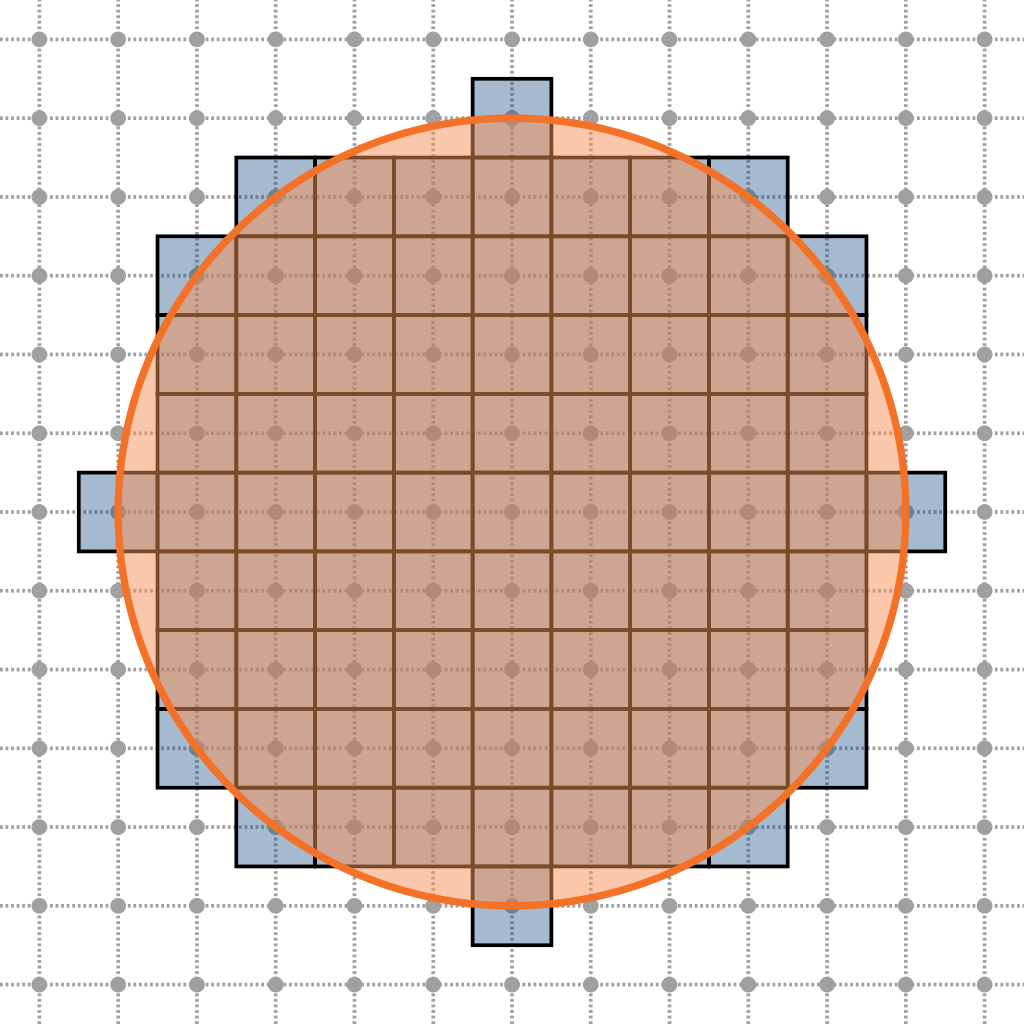
\includegraphics[scale=0.36]{figures/chapter4/digitization/h1.png}
}
\subfloat[$h=0.5$]{
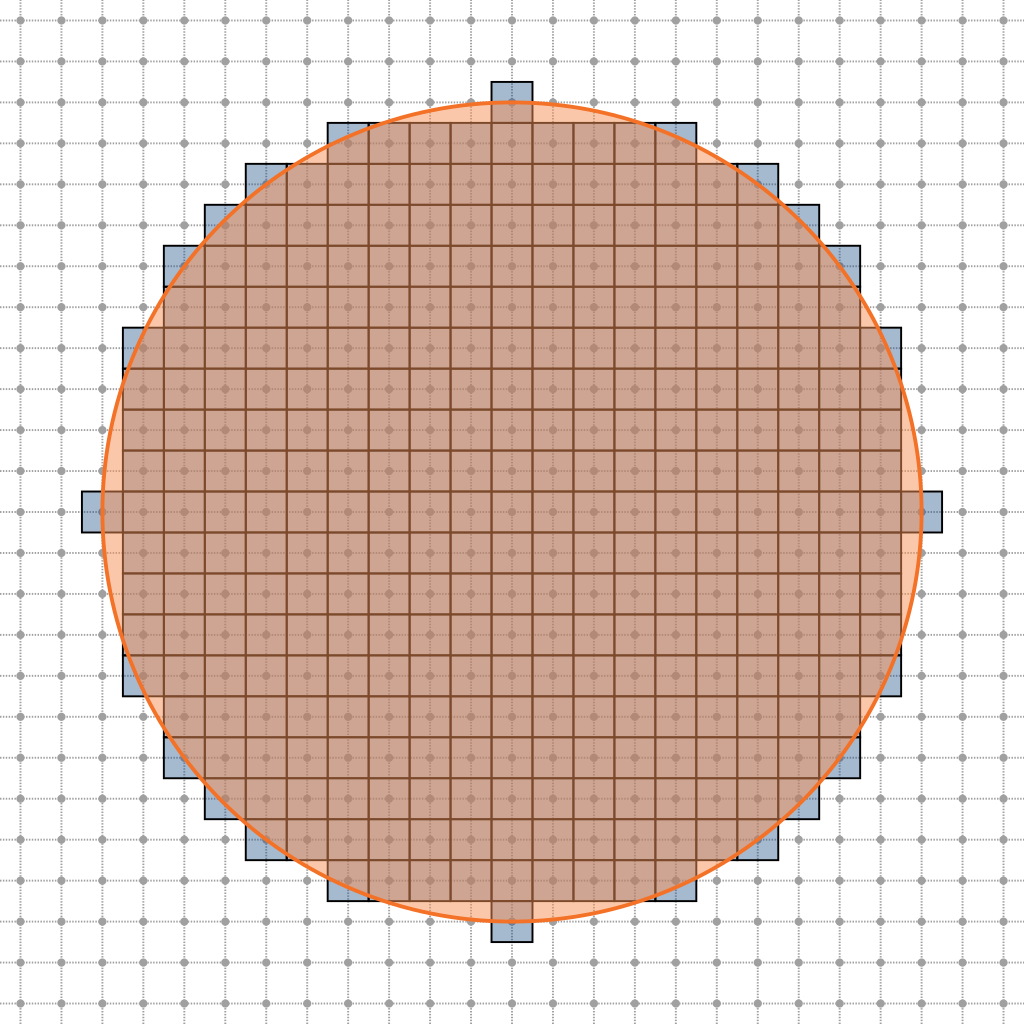
\includegraphics[scale=0.18]{figures/chapter4/digitization/h05.png}
}
\subfloat[$h=0.25$]{
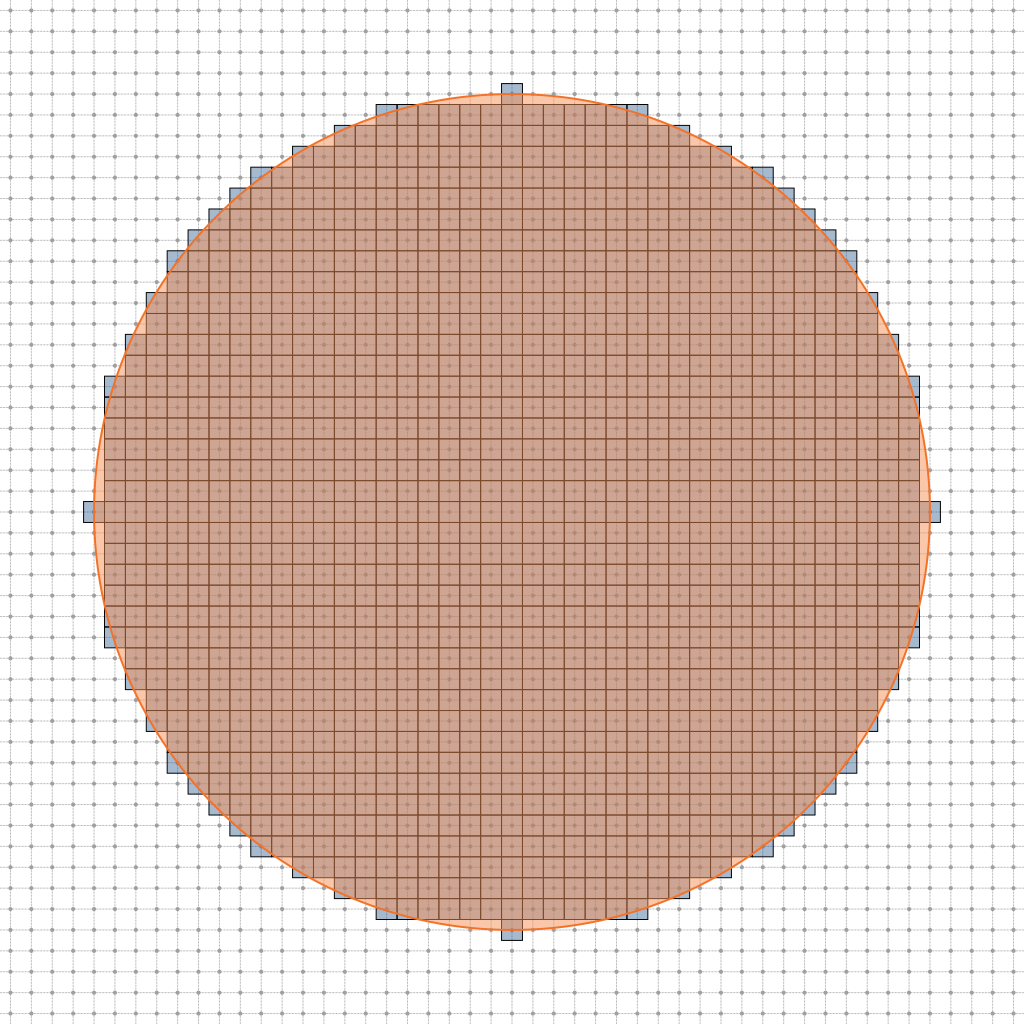
\includegraphics[scale=0.09]{figures/chapter4/digitization/h025.png}
}
\caption{\textbf{Gauss digitization.} Digitization of a ball of radius $5$ in three different resolutions.}
\label{ch4:fig:gauss-digitization}
\end{figure}

In~\cref{ch4:fig:gauss-digitization} we show the Gauss digitization of an Euclidean ball of radius $5$. As one could expect, the Gauss digitization is not adequate for the digitization of lines. In this case, the grid intersection digitization is preferred.

\begin{definition}{Grid intersection digitization}
The grid intersection digitization of a planar curve $\gamma$ is the set of all grid points in the digital grid that are closest (Euclidean distance) to the intersection points of $\gamma$ with the grid lines.
\end{definition}

\begin{figure}
\center
\subfloat[]{
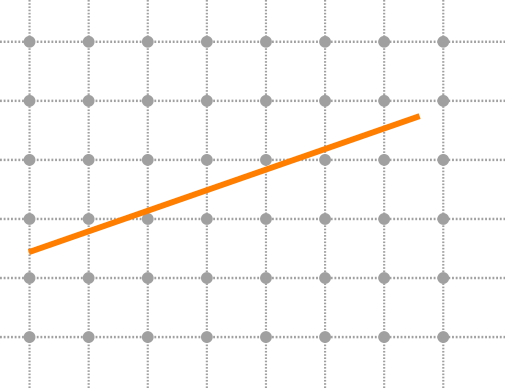
\includegraphics[scale=0.5]{figures/chapter4/digitization/grid-intersection-1.png}
}\hspace{0.5em}
\subfloat[]{
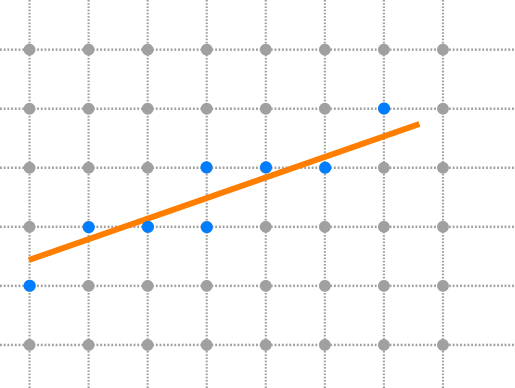
\includegraphics[scale=0.5]{figures/chapter4/digitization/grid-intersection-2.png}
}\hspace{0.5em}
\subfloat[]{
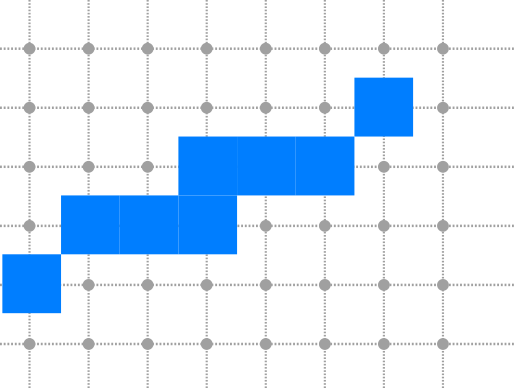
\includegraphics[scale=0.5]{figures/chapter4/digitization/grid-intersection-3.png}
}
\caption{\textbf{Grid intersection digitization.} The Euclidean line is superposed in the digital grid in a); the closest grid points from the intersection with the grid lines are highlighted in blue in b); the grid intersection digitization of the line segment \revision{is given in c}). The digitized segment is $8$-connected.}
\label{ch4:fig:grid-intersection-digitization}
\end{figure}

An illustration of grid intersection digitization is given in~\cref{ch4:fig:grid-intersection-digitization}. The digitization gives us a mapping from continuous objects to its digital grid representation, but an operation in the opposite direction is necessary if we wish to identify geometric primitives. Alternatively, one could define digital geometry primitives, for example, the digital counterpart of a line segment.

\begin{definition}{Digital straight segment (DSS)}
Let $a,b,\mu \in \mathbb{Z}$ such that gcd$(a,b)=1$. The digital straight segment of tangent $a/b$ shifted of $\mu$ from the origin and of width $\varepsilon$ is any subset of $\mathbb{Z}^2$ satisfying~
\begin{align*}
	\{ (x,y) \; | \; \mu \leq ax - by \leq \mu + \varepsilon - 1 \}.
\end{align*}
\end{definition}
\begin{figure}
\center
\subfloat[$\varepsilon= |a| + |b| $]{
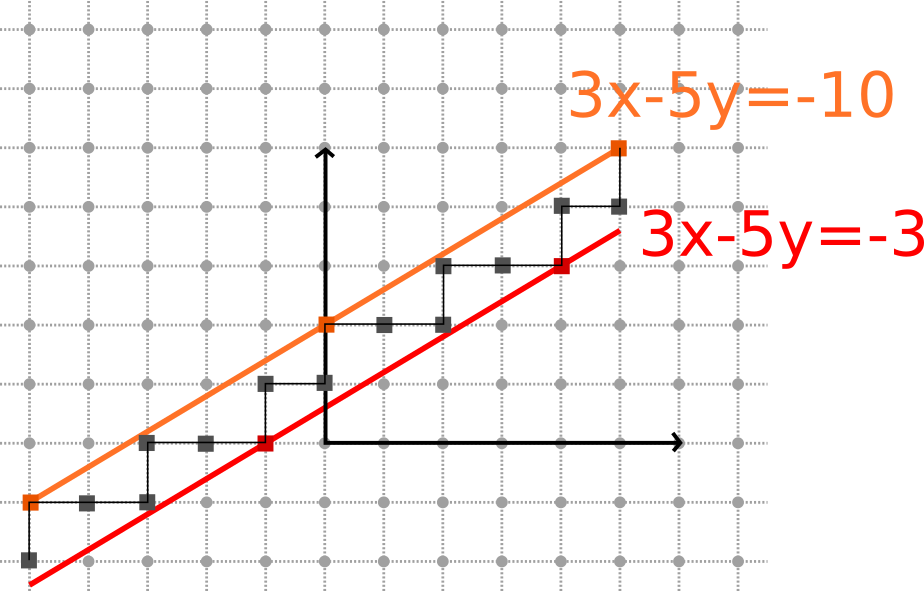
\includegraphics[scale=0.4]{figures/chapter4/dss/four-connected.png}
}
\subfloat[$\varepsilon=\max \{ |a|,|b| \}$]{
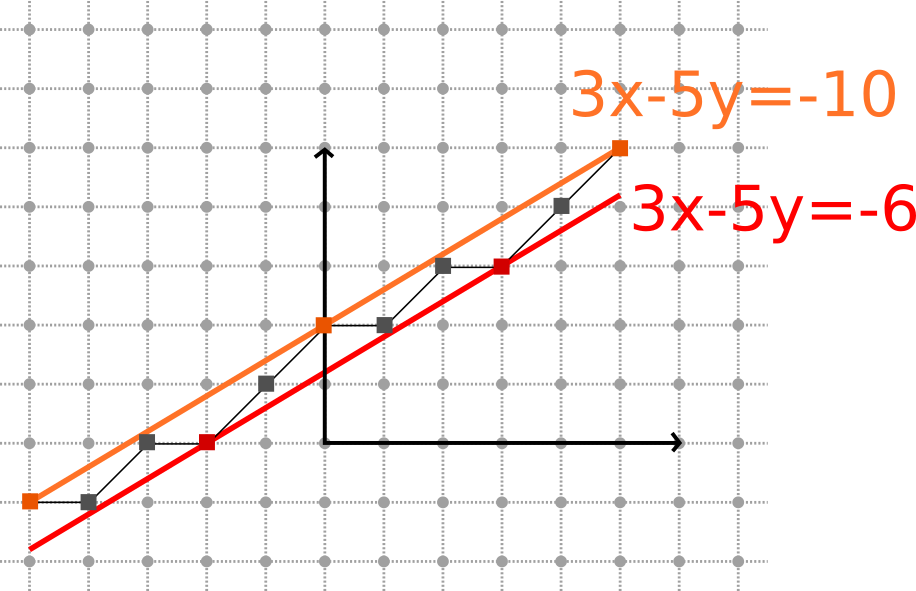
\includegraphics[scale=0.4]{figures/chapter4/dss/eight-connected.png}
}
\caption{\textbf{Digital straight segment.} In a) we have a $4$-connected DSS and in b) a $8$-connected DSS.}
\label{ch4:fig:dss}
\end{figure}

The value of $\varepsilon$ defines the connectivity of the DSS, as illustrated in~\cref{ch4:fig:dss}. In applications, we are going to be interested in the recognition of maximal DSS's, for which linear time algorithms are available~(some of them described in~\cite{klette04digital}, chapter 9). A maximal DSS is a DSS that is not contained in any other DSS. The collection of maximal DSS's in the boundary of a digital set form its~\emph{tangential cover}~(see~\cref{ch4:fig:tangential-cover}). The tangential cover computation is a fundamental step in the computation of convergent estimators of tangent, as we are going to see in the next section.

Finally, we refer to the \emph{digital contour} $\partial_h S$ of $D_h(S)$ as the collection of grid vertices on the boundary of the axis-aligned polygonal shape formed by the grid squares of $D_h(S)$.

\begin{figure}
\center
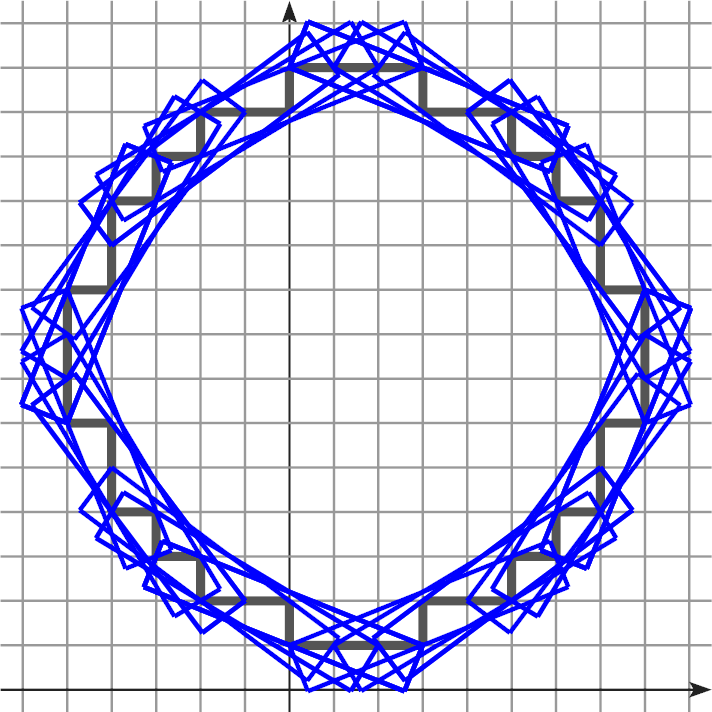
\includegraphics[scale=1]{figures/chapter4/dss/tangential-cover.png}
\caption{\textbf{Tangential conver.} The tangential cover is the collection of all maximal DSS in the digital contour of some digital shape. (Extracted from~\cite{lachaud13multigrid})}
\label{ch4:fig:tangential-cover}
\end{figure}


\subsection{Exact sampling versus digitization}

Let $S$ some regular shape in the plane, for example, a disk of radius $r$. \revision{We wish to} measure the perimeter of $S$, but \revision{let us assume that }we do not know that $S$ is a disk. Additionally, let us assume that we can ask to an oracle for a collection of $n$ points on the boundary of $S$. To make things simple, let us assume that the oracle gives us an ordered sequence of $n$ uniformly spaced points on the boundary of $S$ for a given orientation of $\partial S$. 

\begin{figure}
\center
\subfloat[]{
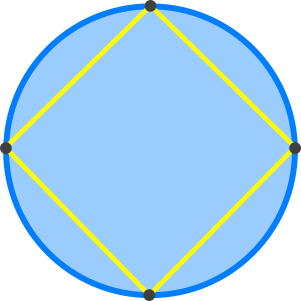
\includegraphics[scale=0.4]{figures/chapter4/exact-sampling/sampling-1.png}
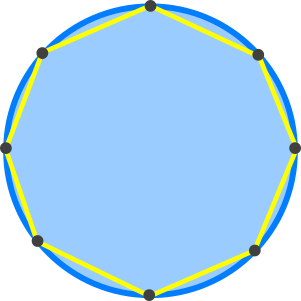
\includegraphics[scale=0.4]{figures/chapter4/exact-sampling/sampling-2.png}
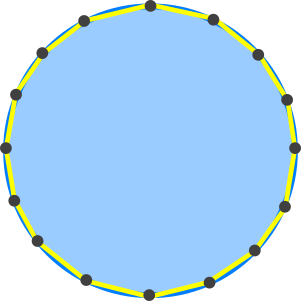
\includegraphics[scale=0.4]{figures/chapter4/exact-sampling/sampling-3.png}
}\hspace{1em}
\subfloat[]{
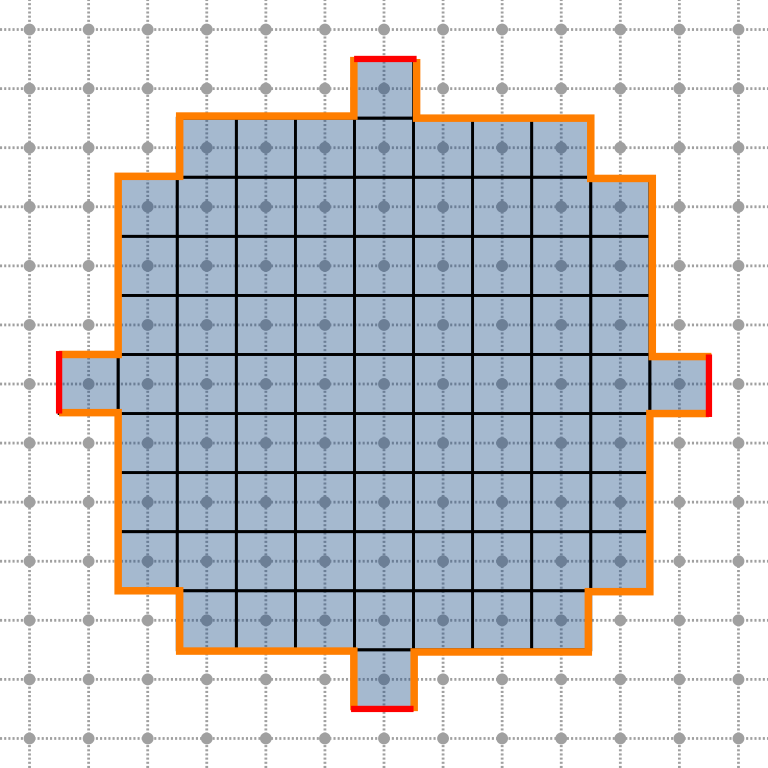
\includegraphics[scale=0.3]{figures/chapter4/exact-sampling/digital-ball-perimeter.png}
}
\caption{\textbf{Exact sampling x digitization.}The perimeter is approximated by the Euclidean polygon formed by $n$ points in the boundary of $S$ in (a). The perimeter is estimated by counting the number of grid edges in (b).}
\label{ch4:fig:exact-sampling-digitization}
\end{figure}

We could estimate the perimeter of $S$ by simply computing the length of the polygon  connecting the $n$ points, i.e., 
\begin{align*}
	L(S) \approx \sum_{i=1}^{n-1}{ \norm{ \overline{p_ip_{i+1}} }}.
\end{align*}
This estimation converges to $2\pi r$ as the number of sampling points increase. Now, let us consider the scenario in which we have a digitization of $S$. The oracle gives us a digitization of $S$ in any resolution $h$. Can we measure the length of $S$ using the same strategy employed in the previous scenario?

Let us say that we engage into estimating the length of $S$ by computing the length of the axis-aligned polygon derived from the digitization of $S$, as illustrated in~\cref{ch4:fig:exact-sampling-digitization}. We assume that the disk is centered at a grid point. It is easy to see that for each quarter of the disk, we have \revision{$2r/h + 1$ horizontal and vertical steps}. Therefore,
\begin{align*}
	\hat{L}(S) &= 4h(2r/h + 1) = 8r + 4h.
\end{align*}
%
The estimator converges to $8r$ as the resolution increases. %Things get more complicated if the disk is not centered at a grid point. 
Several estimators based on the assignment of weights to local configurations were proposed. The BLUE (best linear unbiased) estimator~\cite{dorst87length} \revision{uses a $8$-neighborhood} to estimate perimeter as 
\begin{align*}
	\hat{L}(S) &= h( 0.948 n_i + 1.343 n_d),
\end{align*}
where $n_i$ \revision{is} the number of axis-aligned steps and $n_d$ the number of diagonal steps. Other estimators propose to use an extended set of configurations to cover a higher number of directions, but none of these approaches \revision{can} achieve multigrid convergence, whatever the finite number of configurations employed~\cite{tajine03local}.

This simple example points out that standard discretization strategies of continuous measures or energies, as the one proposed for the discrete elastica in~\cref{chapter:curvature-prior}, do not necessarily extend well in the digital world. The fundamental issue with digital objects is that we have to handle \emph{digitization errors}. We do not have an exact sampling of the continuous object.

\section{Geometric measurements in digital objects}\label{ch4:sec:geometric-measurements}

\subsection{Multigrid convergence and perimeter estimation}

As exemplified in the previous section, geometric measurements in digital objects can be tricky. Intuitively, a good estimator should converge to its continuous counterpart value as the grid resolution is refined. The criteria that formalizes this intuition is the multigrid convergence property.

\begin{definition}{Multigrid convergence}

Let $\mathcal{F}$ a family of shapes in the plane and $Q$ a global measurement (e.g., perimeter, area) on members of $\mathcal{F}$. Additionally, denote $D_h(S)$ a digitization of shape $S$ in a digital grid of resolution $h$. The estimator $\hat{Q}$ of $Q$ is multigrid convergent for the family $\mathcal{F}$ if and only if for every shape $S \in \mathcal{F}$, there exists $h_S > 0$ such that
\begin{align*}
\forall h \leq h_S, \quad |\hat{Q}(D_h(S),h) - Q(S)| \leq \tau_S(h),
\end{align*}
%
where $\tau_S:\mathbb{R}_+\setminus \{0\} \rightarrow \mathbb{R}_+$ is the speed of convergence of $\hat{Q}$ towards $Q$ for $S$.

\end{definition}

In the following, we give some examples of multigrid convergent estimators for perimeter.

\begin{itemize}
	\item[]{\textbf{DSS estimator~\cite{kovalevsky92theoretical}}: It estimates the perimeter by partitioning the digital contours in a sequence of longest DSS's. Starting from any point $p$, it finds the longest DSS starting from $p$ and it repeats the process until all the digital contour is covered. This set of DSS's defines a polygon whose perimeter is the estimated value~(see~\cref{ch4:fig:dss}). It is multigrid convergent for the family of piecewise $3$-smooth convex shapes and also convex polygons.}
	\item[]{\textbf{MLP estimator~\cite{sloboda98approximation}}: It estimates the perimeter of the digital contour as the perimeter of the minimum length polygon that separates interior grid points from exterior grid points~(see~\cref{ch4:fig:mlp}). It is multigrid convergent for all finite convex shapes.}
\end{itemize}

The DSS estimator can be \revision{implemented} in linear-time by using a linear-time DSS recognition algorithm. A linear-time algorithm for the MLP computation is also available~\cite{provenccal09two}.

\begin{figure}
\center
\subfloat[DSS estimator \label{ch4:fig:dss}]
{
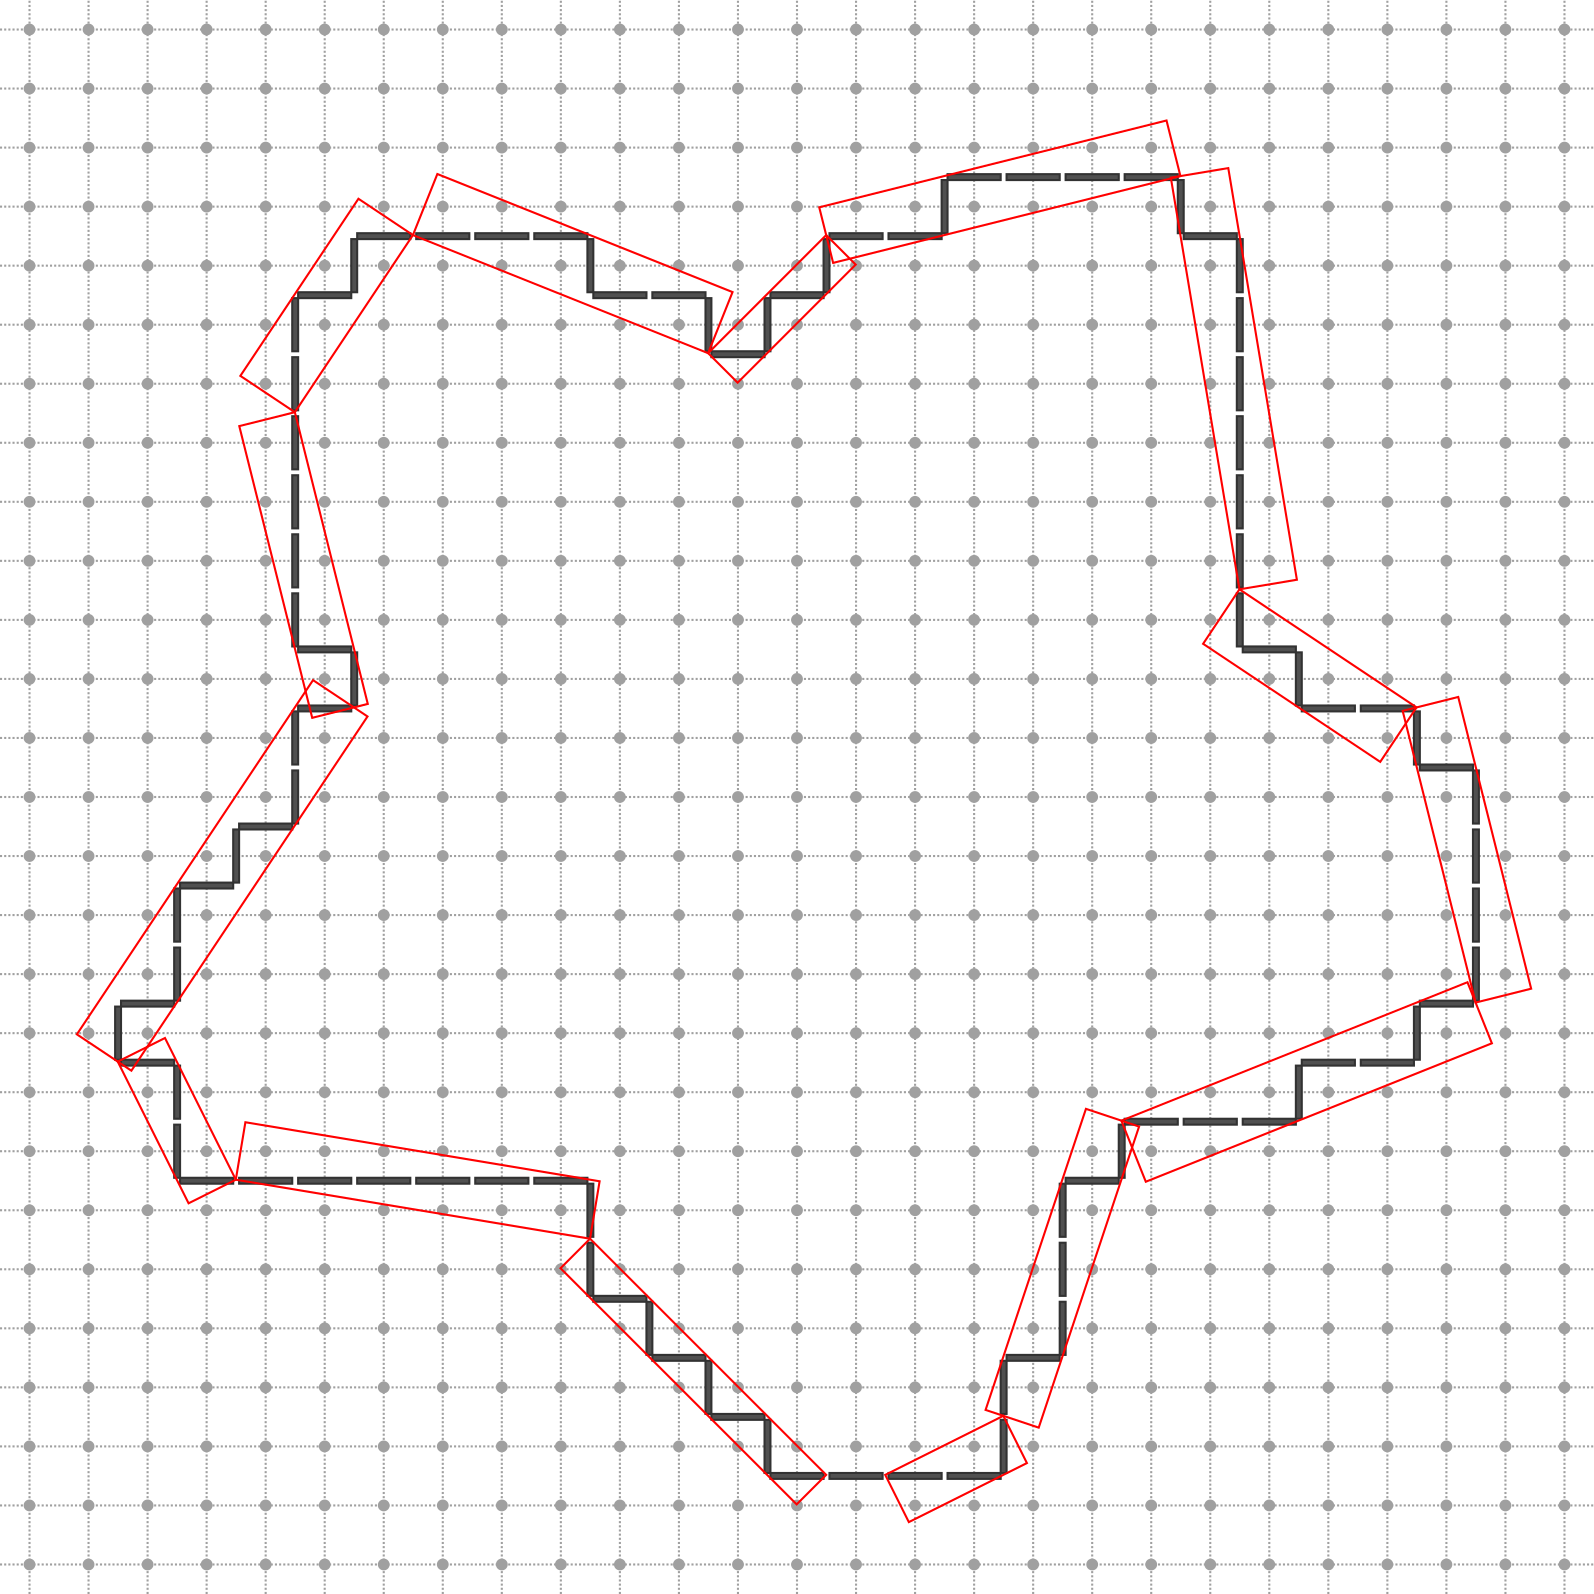
\includegraphics[scale=0.2]{figures/chapter4/perimeter/dss-estimator.png}
}
\subfloat[MLP estimator \label{ch4:fig:mlp} (extracted from~\cite{provenccal09two})]
{
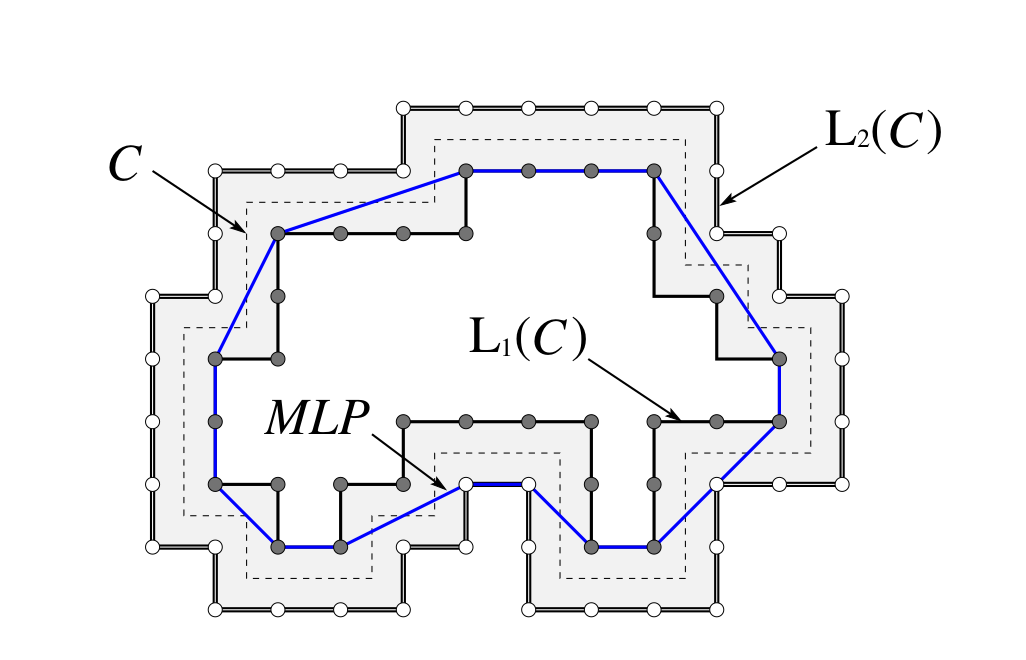
\includegraphics[scale=1.0]{figures/chapter4/perimeter/mlp.png}
}
\caption{\textbf{Multigrid convergent estimators for perimeter.} The perimeter is estimated by sum of the lengths of the recognized DSS in (a). The perimeter is estimated as the length of the minimum length polygon separating inner and outer pixels in (b).}
\end{figure}

Perimeter and area are examples of global properties of shape $S$, i.e., they are not defined at points in $S$ but for the whole shape. A multigrid convergent estimator for area consists in simply counting the number of grid points in its digitization and scale it by $h^2$~\cite{klette00multigrid}. A detailed comparison of several multigrid convergent estimators can be found in~\cite{coeurjolly12multigrid}.


\subsection{Tangent and multigrid convergence of local quantities}

Tangent and curvature are examples of local properties computed along the boundary of some shape $S$ in the plane. We need a slight different definition of multigrid convergence in order to map points of the Euclidean boundary to those in the digital contour.

\begin{definition}{Multigrid convergence for local geometric quantities}
Let $\mathcal{F}$ a family of shapes in the plane and $Q$ a local measurement along the boundary $\partial S$ of $S \in \mathcal{F}$. Additionally, denote $D_h(S)$ a digitization of $S$ in a digital grid of resolution $h$ and $\partial_h S$ its digital contour. The estimator $\hat{Q}$ of $Q$ is multigrid convergent for the family $\mathcal{F}$ if and only if for every shape $S \in \mathcal{F}$, there exists $h_S > 0$ such that the estimate $\hat{Q}(D_h(S),p,h)$ is defined for all $p \in \partial_h S$ with $0 < h < h_S$, and for any $x \in \partial S$,
\begin{align*}
	\forall p \in \partial_h S \text{ with } \norm{p-x}_{\infty} \leq h,\quad | \hat{Q}(D_h(S),p,h) - Q(S,x) | \leq \tau_S(h),	
\end{align*}
where $\tau_S:\mathbb{R}_+\setminus \{0\} \rightarrow \mathbb{R}_+$ has null limit at $0$. This function defines the speed of convergence of $\hat{Q}$ towards $Q$ for $S$.
\end{definition}


The $\lambda$-MST tangent estimator~\cite{lachaud07tangent} computes the tangential cover of $D_h(S)$ and then estimates the tangent direction at point $p \in \partial_h S$ as a weighted combination of the tangents directions $\tan^{-1}(a/b)$  of maximal DSS $(a,b,\mu,\varepsilon)$ passing through $p$. We recall that we defined digital contours as a collection of grid vertices, but we can always interpret them as grid points. It is enough to translate every grid vertex by $h(0.5,0.5)$.

For a given order in the points of $\partial_h S$, a maximal DSS starting at $p_i$ and ending at $p_j$ is denoted $C_{ij}$. For each $p_k \in \partial_h S$, let $\mathcal{C}(p_k)$ be the set of maximal DSS's passing through $p_k$. The eccentricity of a point $p_k$ is defined as
\begin{align*}
	e(p_k) &= \left\{ \begin{array}{cc}
	\frac{|k-j|}{|i-j|}, & \text{if } C_{ij} \in \mathcal{C}(p_k) \\
	0, & \text{otherwise}.
	\end{array}\right.
\end{align*}
%
The tangent direction at $p_k$ is estimated as
\begin{align*}
	\hat{\theta}(p_k) &= \frac{ \sum_{C_{ij} \in \mathcal{C}(p_k) }{ \lambda( e(p_k) ) \tan^{-1}(a_{ij}/b_{ij}) } }{ \sum_{C_{ij} \in \mathcal{C}(p_k) }{ \lambda( e(p_k) )} },
\end{align*}
%
where $\lambda$ is a mapping from $[0,1]$ to $\mathbb{R}^+$ with $\lambda(0)=\lambda(1)=0$ and $\lambda > 0$ elsewhere. The $\lambda$-MST estimator is multigrid convergent for the family of convex shapes that are twice differentiable with continuous curvature. The convergence speed is of $O(h^{1/3})$~\cite{lachaud07tangent}.

The $\lambda$-MST estimator can be used to estimate the contribution of each grid edge to the perimeter of the shape, the so-called \emph{elementary length}. Let $\{\vec{e}_i\}$ be the collection of grid edges (vectors) in the digital contour of $D_h(S)$. We compute the $\lambda$-MST estimator for the sequence of points formed by the center points $\dot{\vec{e}}_i$ of each $\vec{e}_i$. The elementary length is defined as
\begin{align*}
\hat{\ell}(\vec{e}_i) &= \big( \sin( \hat{\theta}(\dot{\vec{e}}_i) ), \cos( \hat{\theta}(\dot{\vec{e}}_i) ) \big) \cdot \vec{e_i}.
\end{align*}
%
One can integrate the elementary length to obtain a multigrid convergent estimator for the perimeter of $S$. More generally, given a measurement $g$ in $\partial S$ and a multigrid convergent estimator $\hat{g}$ of $g$ in $\partial_h S$, the expression
\begin{align*}
	\sum_{\vec{e}_i \in \partial_h S}{ \hat{g}(\vec{e}_i) \hat{l}(\vec{e}_i)},
\end{align*}
%
is a multigrid convergent estimator for the energy~\cite{lachaud06hdr}
\begin{align*}
	\int_{\partial S}{ g ds }.
\end{align*}
%
%
%
\subsection{Multigrid convergent estimators of curvature}

Analogously to digital straight segments, the \emph{digital circular arc} is the digital counterpart of a circular arc. For any $C \in \partial_h S$, a grid point $p$ is an interior (exterior) point of $C$ if $p \in D_h S$ ($p \notin D_h S$) and there exists a grid edge in $C$ that is incident to the grid square corresponding to $p$.

\begin{definition}{Digital circular arc} 
A segment $C \in \partial_h S$ is a digital circular arc if and only if the interior and exterior grid points of $C$ are circularly separable, i.e., there exists an Euclidean circle that either encloses the interior points without enclosing any exterior points or that encloses the exterior points without enclosing any interior point.
\end{definition}

An illustration is given in~\cref{ch4:fig:digital-circular-arc}.The Maximal Digital Circular Arcs estimator (MDCA)~\cite{roussillon11mdca} estimates the curvature at point $p \in \partial_h S$ as the inverse of the radius of the most centered digital circular arc that contains $p$. The MDCA estimator is multigrid convergent for the family of convex shapes in the plane with continuous, strictly positive and bounded curvature. An alternative is the $\lambda$-MDCA estimator~\cite{schindele17mdca}, which follows the same rational of the $\lambda$-MST. The $\lambda$-MDCA has been proven multigrid convergent for the same family of convex shapes with continuous curvature. It converges with speed $O(h^{1/3})$.


\begin{figure}
\center
\subfloat[Digital circular arc (extracted from~\cite{roussillon11mdca} ) \label{ch4:fig:digital-circular-arc}]{
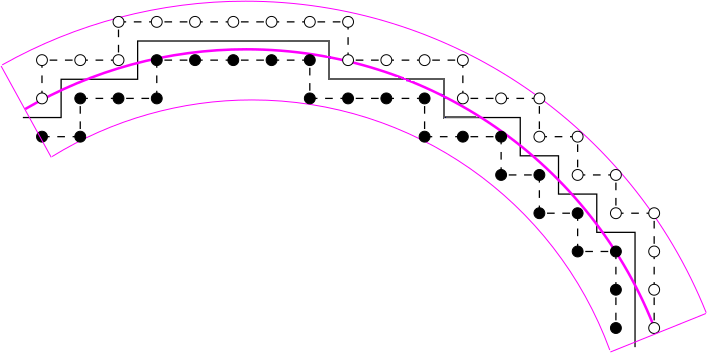
\includegraphics[scale=0.2]{figures/chapter4/curvature/digital-circular-arc.png}
}\hspace{1em}
\subfloat[II estimator (extracted from~\cite{coeurjolly13integral} ) \label{ch4:fig:ii-estimator}]{
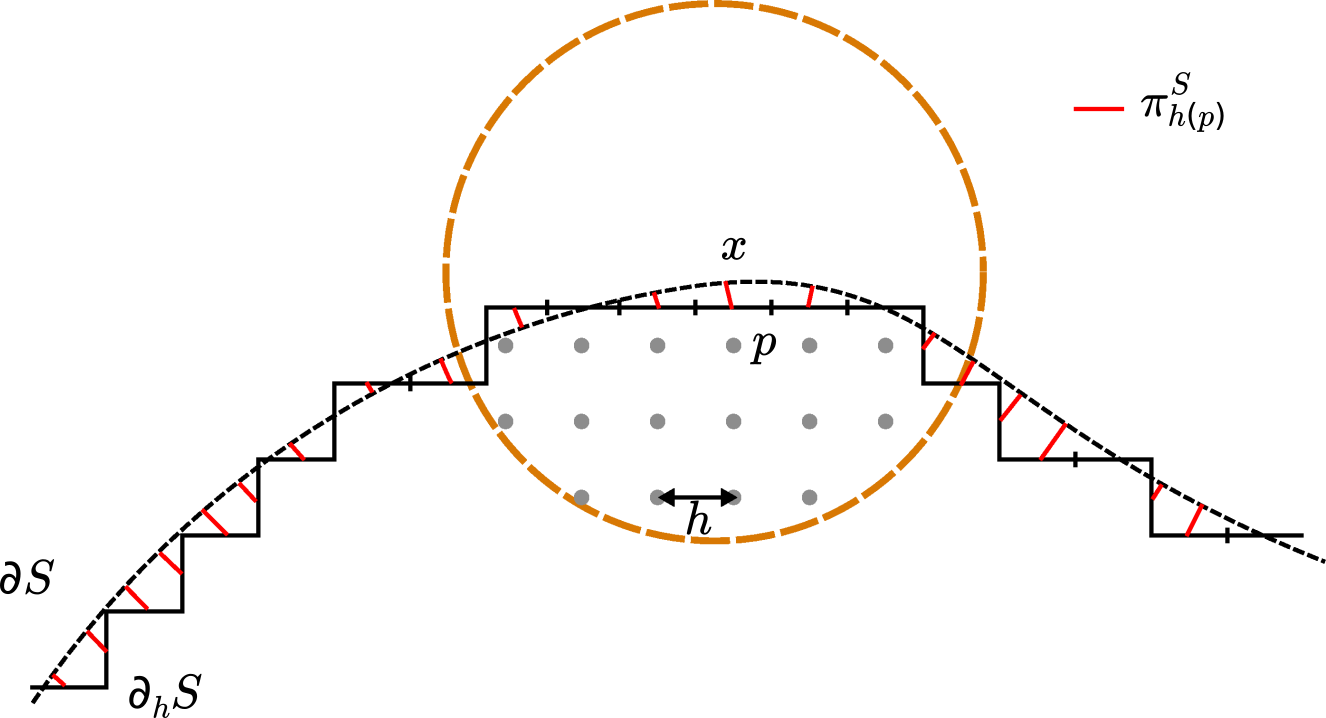
\includegraphics[scale=0.36]{figures/chapter4/curvature/ii-digital-contour.png}
}
\caption{\textbf{Curvature estimation.} The digital circular arc separates the interior grid points (black) from the exterior grid points (white) in (a). The back-projection operator maps digital grid points to points in $\partial S$ in (b). }
\end{figure}

The next curvature estimator is based on the concept of integral invariants. Generally speaking, an invariant is a function whose value is unaffected by the action of some group on the elements of its domain. The curvature, for example, is an invariant for shapes in $\mathbb{R}^2$ with respect to the Euclidean group of rigid transformations. However, curvature is a second order differential invariant and its computation is very sensitive to noise. In the digital grid, the issues appearing in tangent estimation are amplified for curvature estimation.

An integral invariant, on the other hand, is a value computed via integration and one can expect \revision{more robustness} to noise. In the context of digital estimation, an integral invariant is attractive because we have already a very simple multigrid convergent estimator to estimate the area. In~\cite{manay04intinvariant}, the authors define the integral area invariant and link it with the measurement of curvature

\begin{definition}{Integral area invariant}
  Let $S \subset \mathbb{R}^2$ and $B_r(x)$ the Euclidean ball of radius $r$ centered at point $x$. Further, let  $\mathbf{1}_S(\cdot)$ be the characteristic function of $S$. The integral area invariant $\sigma_{S,r}(\cdot)$ is
  defined as
  \begin{align*}
    \forall x \in \partial S, \quad \sigma_{S,r}(x) = \int_{B_r(x)}{ \mathbf{1}_S(y) dy}.
  \end{align*}
\end{definition}
%
%
The value $\sigma_{S,r}(x)$ is the area of the intersection of the ball $B_r(x)$ with shape $S$. By approaching the shape at point $x \in S$, one can rewrite the intersection area $\sigma_{S,r}(x)$ in the form of the Taylor expansion~\cite{pottman09intinvariant}:
\begin{align*}
  \sigma_{S,r}(p) = \frac{\pi}{2}r^2 - \frac{\kappa(S,x)}{3}r^3 + O(r^4),
\end{align*}
%
where $\kappa(S,x)$ is the curvature of $S$ at point $x$. By isolating $\kappa$ we can define a curvature estimator
%	
\begin{align}
  \tilde{\kappa}(x) \coloneqq \frac{3}{r^3}\left( \frac{\pi r^2}{2} - \sigma_{S,r}(x) \right).
  \label{ch4:eq:curvature_approximation}
\end{align}
%
In~\cite{coeurjolly13integral}, the authors combine the approximation~\cref{ch4:eq:curvature_approximation} and the estimator of area to define a multigrid convergent estimator for the curvature (see~\cref{ch4:fig:ii-estimator}).

\begin{definition}{Integral Invariant Curvature Estimator}
  Let $D_h(S)$ a digitization of $S \subset \mathbb{R}^2$. The integral invariant curvature estimator is defined for every point $p \in \partial_h S$ as
  \begin{align*}
    \hat{\kappa}_{r}(D_h(S),p,h) \coloneqq \frac{3}{r^3} \left( \frac{\pi r^2}{2} - \widehat{\text{Area}} \left( D_h\big( B_{r} ( p ) \big) \cap D_h(S), h \right) \right).
    %% \hat{\kappa}_{r}(D,x,h) \coloneqq \frac{3}{r^3} \left( \frac{\pi r^2}{2} - \widehat{Area} \left( B_{r/h} ( \frac{1}{h} \cdot x ) \cap D, h \right) \right),
  \end{align*}
\end{definition}
%
where $\widehat{\text{Area}}( D,h )$ estimates the area of $D$ by counting its grid points and then scaling them by $h^2$. \daniel{This estimator is multigrid convergent for the family of compact shapes in the plane with $3$-smooth boundary. It converges with speed $O(h^\frac{1}{3})$ for radii chosen as $r=\Theta(h^\frac{1}{3})$~\cite{lachaud17robust}.}

\section{Conclusion}

In imaging problems it is very rare to have a mathematical description of the objects in the scene. If we wish to measure geometric properties on these objects, we have to deal with its digitization error. In contrast with exact sampling, whose points can be located everywhere in $\mathbb{R}^2$, the digital grid restricts the sampling to a subset of $h\mathbb{Z}^2$. In this chapter, we have shown that we cannot extend standard discretization strategies to do geometric measurements of digital objects. Instead, we should study the problem from the point of view of digital geometry and the multigrid convergence property.


%\section{Three types of error}
%
%One may divide a problem solving task in three general steps: i) problem statement; ii) model proposal; and iii) solution. In fortunate occasions, the proposed model can be solved analytically and error concerns will arise in the eventual use of computers to do automatic computations, in which we have the \emph{machine error representation}. That is the case, for example, when we have to solve a system of linear equations.
%
%If we propose to solve, instead, a system of non-linear equations, we likely have to use a numerical method such as Newton-Rapson. In this case, we are susceptible to not only  machine errors but also to \emph{convergence errors} of the numerical method.
%
%Next, if the proposed model involves to solve a partial differential equation such as the one arising from the heat equation, we also have the discretization error.
%
%
%\begin{enumerate}
%	\item{We have \emph{complete} knowledge of the mathematical objects involved;}
%	\item{We have an \emph{exact} sampling of the mathematical objects involved;}
%	\item{We have an \emph{approximate} sampling of the mathematical objects involved}
%\end{enumerate}
%
%In the first case, there is no much change. In the second case, the quality of solution may depend of the number of samples. Take for example the discrete elastica in chapter 3. The error with respect with the continuous elastica can be arbitrarily small as long a sufficient number of curve samplings are employed.
%
%The last case is the one which digital geometry is mainly concerned.
%
%\section{Continuous, discrete and digital}
%
%The concept of infinite and continuity are among the most powerful in mathematics. Optimization, differential equations 
%
%The infinitely thin and infinitely long model of a line is an abstraction of Euclidean geometry. Likewise, the dimensionless concept of a point does not find parallel in nature.  Nonetheless, the idea of infinite and continuous objects are powerful in science, in particular mathematics. But some 
%
%It is curious that we have more knowledge 



